\documentclass[tikz,border=10pt]{standalone}
\usepackage{amsmath,amssymb}
\usepackage{xcolor}
\usepackage{tikz}
\usetikzlibrary{positioning,calc,arrows.meta}

% ---------------- palette (colorblind-friendly) ----------------
\definecolor{netblue}{RGB}{31,119,180}
\definecolor{uncorange}{RGB}{216,100,20}
\definecolor{calteal}{RGB}{22,155,122}
\definecolor{fwd}{RGB}{65,65,65}

\tikzset{
  block/.style={draw=gray!65,fill=gray!7,rounded corners=2.5pt,align=center,inner sep=4pt,line width=0.7pt},
  oblock/.style={draw=netblue!85,fill=netblue!6,rounded corners=2.5pt,align=center,inner sep=4pt,line width=0.95pt},
  ublock/.style={draw=uncorange!90,fill=uncorange!6,rounded corners=2.5pt,align=center,inner sep=4pt,line width=0.95pt},
  lossnode/.style={circle,draw=gray!65,fill=white,minimum size=7.4mm,inner sep=0pt,line width=0.7pt,font=\footnotesize},
  sgnode/.style={circle,draw=gray!60,fill=gray!20,minimum size=7mm,inner sep=0pt,font=\footnotesize\bfseries,line width=0.7pt},
  sgbadge/.style={rectangle,rounded corners=1.5pt,draw=gray!55,fill=gray!18,inner sep=2.2pt,font=\tiny\bfseries,line width=0.5pt,text=black},
  smallhead/.style={draw=gray!65,fill=gray!8,rounded corners=1.5pt,minimum width=9.5mm,minimum height=5.6mm,inner sep=0pt,font=\footnotesize,line width=0.7pt},
  flow/.style={-{Latex[length=2.1mm,width=1.9mm]},line width=0.85pt,fwd},
  gradw/.style={-{Latex[length=2.8mm,width=2.5mm]},line width=1.3pt,netblue},
  gradth/.style={-{Latex[length=2.8mm,width=2.5mm]},line width=1.3pt,uncorange},
  dashcal/.style={-{Latex[length=2mm,width=1.8mm]},dashed,line width=0.9pt,calteal},
}

\begin{document}
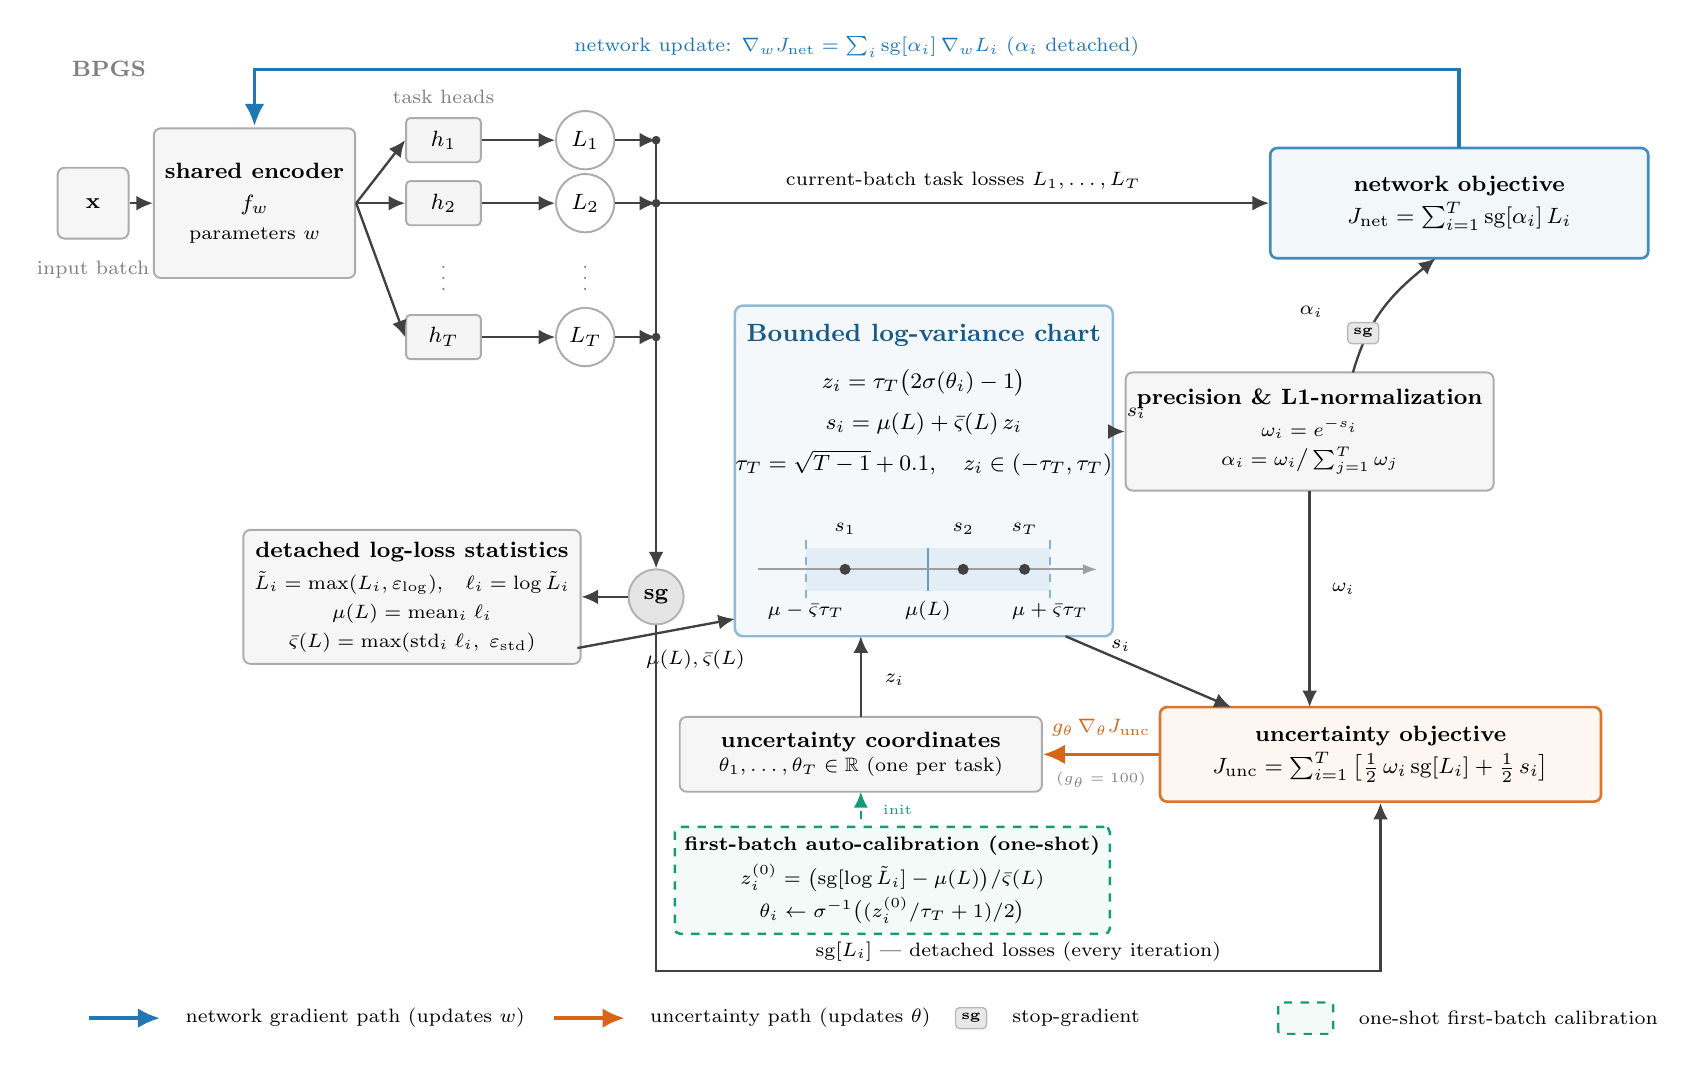
\begin{tikzpicture}[font=\footnotesize]

% ================= bounded chart panel (background) =================
\filldraw[fill=netblue!5,draw=netblue!50,rounded corners=3pt,line width=0.9pt]
  (8.7,2.5) rectangle (13.5,6.7);

% ================= forward pass =================
\node[block,minimum width=9mm,minimum height=9mm] (input) at (0.55,8.0) {$\mathbf{x}$};
\node[font=\scriptsize,gray] at (0.55,7.15) {input batch};

\node[block,minimum width=19mm,minimum height=19mm] (enc) at (2.6,8.0)
  {\textbf{shared encoder}\\[2pt] $f_{w}$\\[1pt] {\scriptsize parameters $w$}};

\node[smallhead] (h1) at (5.0,8.8) {$h_1$};
\node[smallhead] (h2) at (5.0,8.0) {$h_2$};
\node[font=\scriptsize,gray] at (5.0,7.15) {$\vdots$};
\node[smallhead] (hT) at (5.0,6.3) {$h_T$};
\node[font=\scriptsize,gray] at (5.0,9.35) {task heads};

\node[lossnode] (L1) at (6.8,8.8) {$L_1$};
\node[lossnode] (L2) at (6.8,8.0) {$L_2$};
\node[font=\scriptsize,gray] at (6.8,7.15) {$\vdots$};
\node[lossnode] (LT) at (6.8,6.3) {$L_T$};

\draw[flow] (input.east) -- (enc.west);
\draw[flow] (enc.east) -- (h1.west);
\draw[flow] (enc.east) -- (h2.west);
\draw[flow] (enc.east) -- (hT.west);
\draw[flow] (h1.east) -- (L1.west);
\draw[flow] (h2.east) -- (L2.west);
\draw[flow] (hT.east) -- (LT.west);

% ---- loss bus ----
\draw[flow] (L1.east) -- (7.7,8.8);
\draw[flow] (L2.east) -- (7.7,8.0);
\draw[flow] (LT.east) -- (7.7,6.3);

% ================= stop-gradient node + statistics =================
\node[sgnode] (sgn) at (7.7,3.0) {sg};

\node[block,minimum width=42mm,minimum height=17mm] (stats) at (4.6,3.0)
  {\textbf{detached log-loss statistics}\\[2pt]
   {\scriptsize $\tilde L_i=\max(L_i,\varepsilon_{\log})$,~~ $\ell_i=\log\tilde L_i$}\\[1pt]
   {\scriptsize $\mu(L)=\mathrm{mean}_i\;\ell_i$}\\[1pt]
   {\scriptsize $\bar\varsigma(L)=\max(\mathrm{std}_i\;\ell_i,\;\varepsilon_{\mathrm{std}})$}};

\draw[flow] (sgn.west) -- (stats.east);
\draw[flow] (6.7,2.35) -- (8.7,2.72);
\node[font=\scriptsize] at (8.2,2.2) {$\mu(L),\bar\varsigma(L)$};

% ================= chart internals =================
\node[font=\small\bfseries,text=netblue!75!black] at (11.1,6.32) {Bounded log-variance chart};
\node at (11.1,5.72) {$z_i=\tau_T\big(2\sigma(\theta_i)-1\big)$};
\node at (11.1,5.20) {$s_i=\mu(L)+\bar\varsigma(L)\,z_i$};
\node at (11.1,4.70) {$\tau_T=\sqrt{T-1}+0.1,\quad z_i\in(-\tau_T,\tau_T)$};

\fill[netblue!13] (9.6,3.08) rectangle (12.7,3.62);
\draw[dashed,netblue!55,line width=0.6pt] (9.6,2.98)  -- (9.6,3.72);
\draw[dashed,netblue!55,line width=0.6pt] (12.7,2.98) -- (12.7,3.72);
\draw[netblue!70,line width=0.8pt] (11.15,3.08) -- (11.15,3.62);
\draw[-{Latex[length=1.8mm]},gray!75,line width=0.7pt] (9.0,3.35) -- (13.3,3.35);

\node[font=\scriptsize] at (9.6,2.82)  {$\mu-\bar\varsigma\tau_T$};
\node[font=\scriptsize] at (11.15,2.82) {$\mu(L)$};
\node[font=\scriptsize] at (12.7,2.82) {$\mu+\bar\varsigma\tau_T$};

\fill[fwd] (10.1,3.35)  circle (0.07);
\fill[fwd] (11.6,3.35)  circle (0.07);
\fill[fwd] (12.38,3.35) circle (0.07);
\node[font=\scriptsize] at (10.1,3.86)  {$s_1$};
\node[font=\scriptsize] at (11.6,3.86)  {$s_2$};
\node[font=\scriptsize] at (12.38,3.86) {$s_T$};

% ================= uncertainty coordinates + calibration =================
\node[block,minimum width=46mm,minimum height=9.5mm] (theta) at (10.3,1.0)
  {\textbf{uncertainty coordinates}\\[-1pt]
   {\scriptsize $\theta_1,\dots,\theta_T\in\mathbb{R}$ (one per task)}};

\draw[flow] (10.3,1.475) -- (10.3,2.5);
\node[font=\scriptsize,anchor=west] at (10.48,1.95) {$z_i$};

\node[draw=calteal,dashed,fill=calteal!5,rounded corners=2pt,line width=0.9pt,
      align=center,inner sep=3.5pt,font=\scriptsize] (calib) at (10.7,-0.6)
  {\textbf{first-batch auto-calibration (one-shot)}\\[2pt]
   $z_i^{(0)}=\big(\mathrm{sg}[\log\tilde L_i]-\mu(L)\big)/\bar\varsigma(L)$\\[1pt]
   $\theta_i\leftarrow\sigma^{-1}\big((z_i^{(0)}/\tau_T+1)/2\big)$};

\draw[dashcal] (10.3,0.18) -- (10.3,0.525);
\node[font=\tiny,text=calteal,anchor=west] at (10.46,0.3) {init};

% ================= precision & normalization =================
\node[block,minimum width=40mm,minimum height=15mm] (prec) at (16.0,5.1)
  {\textbf{precision \& L1-normalization}\\[2pt]
   {\scriptsize $\omega_i=e^{-s_i}$}\\[1pt]
   {\scriptsize $\alpha_i=\omega_i\big/\sum_{j=1}^{T}\omega_j$}};

\draw[flow] (13.5,5.1) -- (prec.west);
\node[font=\scriptsize] at (13.8,5.33) {$s_i$};

% ================= split objectives =================
\node[oblock,minimum width=48mm,minimum height=14mm] (Jnet) at (17.9,8.0)
  {\textbf{network objective}\\[2pt]
   {\footnotesize $J_{\mathrm{net}}=\sum_{i=1}^{T}\mathrm{sg}[\alpha_i]\,L_i$}};

\node[ublock,minimum width=56mm,minimum height=12mm] (Junc) at (16.9,1.0)
  {\textbf{uncertainty objective}\\[2pt]
   {\footnotesize $J_{\mathrm{unc}}=\sum_{i=1}^{T}\big[\tfrac{1}{2}\,\omega_i\,\mathrm{sg}[L_i]+\tfrac{1}{2}\,s_i\big]$}};

% bus -> J_net (raw losses, not detached)
\draw[flow] (7.7,8.0) -- (Jnet.west);
\node[font=\scriptsize] at (11.6,8.28) {current-batch task losses $L_1,\dots,L_T$};

% alpha -> J_net with stop-gradient badge
\draw[flow] (16.55,5.85) .. controls (16.75,6.55) and (17.05,6.85) .. (17.6,7.3);
\node[sgbadge] at (16.68,6.35) {sg};
\node[font=\scriptsize] at (16.02,6.62) {$\alpha_i$};

% chart outputs into J_unc
\draw[flow] (12.9,2.5) -- (15.0,1.6);
\node[font=\scriptsize] at (13.6,2.38) {$s_i$};
\draw[flow] (16.0,4.35) -- (16.0,1.6);
\node[font=\scriptsize,anchor=west] at (16.16,3.1) {$\omega_i$};

% detached losses into J_unc
\draw[flow] (sgn.south) -- (7.7,-1.75) -| (Junc.south);
\node[font=\scriptsize] at (12.3,-1.5) {$\mathrm{sg}[L_i]$ — detached losses (every iteration)};

% ================= gradient updates =================
\draw[gradth] (Junc.west) -- (theta.east);
\node[font=\scriptsize,text=uncorange] at (13.35,1.34) {$g_\theta\,\nabla_\theta J_{\mathrm{unc}}$};
\node[font=\tiny,gray] at (13.35,0.68) {$(g_\theta=100)$};

\draw[gradw] (17.9,8.7) -- (17.9,9.7) -- (2.6,9.7) -- (2.6,8.98);
\node[font=\scriptsize,text=netblue] at (10.25,9.98)
  {network update: $\nabla_w J_{\mathrm{net}}=\sum_i \mathrm{sg}[\alpha_i]\,\nabla_w L_i$  ($\alpha_i$ detached)};

\node[font=\footnotesize\bfseries,gray] at (0.75,9.7) {BPGS};

% ================= bus junctions (drawn last) =================
\fill[fwd] (7.7,8.8) circle (0.055);
\fill[fwd] (7.7,8.0) circle (0.055);
\fill[fwd] (7.7,6.3) circle (0.055);
\draw[flow] (7.7,8.8) -- (sgn.north);

% ================= legend =================
\draw[gradw] (0.5,-2.35) -- (1.4,-2.35);
\node[font=\scriptsize,anchor=west] at (1.6,-2.35) {network gradient path (updates $w$)};
\draw[gradth] (6.4,-2.35) -- (7.3,-2.35);
\node[font=\scriptsize,anchor=west] at (7.5,-2.35) {uncertainty path (updates $\theta$)};
\node[sgbadge] at (11.7,-2.35) {sg};
\node[font=\scriptsize,anchor=west] at (12.1,-2.35) {stop-gradient};
\draw[draw=calteal,dashed,fill=calteal!5,rounded corners=1pt,line width=0.8pt]
  (15.6,-2.55) rectangle (16.3,-2.15);
\node[font=\scriptsize,anchor=west] at (16.5,-2.35) {one-shot first-batch calibration};

\end{tikzpicture}
\end{document}